\documentclass[fontsize=11pt]{article}
\usepackage{amsmath}
\usepackage[utf8]{inputenc}
\usepackage[margin=0.75in]{geometry}
\usepackage{hyperref}
\usepackage{graphicx}

\title{CSC110 Project Report: US Snowfall vs. Global Land-Ocean Temperature Index}
\author{Gabe Guralnick, Matthew Toohey, Monica Di Gennaro, Nathan Hansen}
\date{Monday, December 14, 2020}

\begin{document}
\maketitle

\section*{Problem Description and Research Question}

In the past few decades, climate change has made widespread impacts on many of the earth's ecosystems.
As temperatures are increasing, flora and fauna across the globe that have never experienced the temperatures we are now seeing, on a regular basis, that they are reacting in unpredictable ways.
For example, the Arctic ice caps are melting, which is causing rising sea levels and disrupting weather systems. Migratory species, such as whales, birds, and butterflies have also been affected due to their dependency on the temperature, vegetation, weather, and more on their surrounding environment. Moreover, third world countries have been experiencing an increase in deaths due to heat-related illnesses, such as heat stress and heat stroke, which is in direct correlation to climate change. A more familiar phenomenon to people in developed countries would be a change in precipitation, which could also be seen as the most known consequence of progressing global warming. In particular, the environmental system of snowfall is one aspect that has likely been affected by rising temperatures.
Areas which once received large amounts of snowfall and therefore were adapted to the weather and desirable to tourists for activities like skiing and snowboarding now receive much less snow, and areas whose winter weather was previously more mild now receive much more. A paper written in March 2018 showed that over 33\% of snow monitoring sites in the western United States have shown statistically significant and concerning declines in the past 14 years (Mote et al., 2018).
Since snow requires much colder temperatures in order to form instead of simply becoming rain, increased temperatures due to climate change have decreased the amount of snowfall in recent years as climate change has rapidly progressed. For our group's project proposal, we will be investigating the widespread effects of climate change within the United States, specifically its impact on snowfall.\\

\textbf{Research question: ``How have increasing global temperatures affected the regional impact of snowfall in the US?"}

\section*{Data-Set Description}

There are two main data-sets that we used for this report.
The first is the NASA Temperature Index data-set (NASA/GISS, 2019).
This data-set includes Land-Ocean Temperature Index data from 1880 to 2019.
Each year has a both a \texttt{No\_Smoothing} and \texttt{Lowess} (locally weighted scatter plot smoothing) values.
A ``Land-Ocean Temperature Index" is a combined index of surface air temperature data measured by weather stations, and sea surface temperatures, measured by ship, buoy, and satellite reports, as explained by NASA's GISTEMP FAQ page (Schmunk, 2019).
The data-set was provided as a \texttt{.txt} file, but we converted it to a \texttt{.csv} to keep our formats consistent between both data-sets. We used all three columns of this data-set for our project: Year, No\_Smoothing, and Lowess. The Year column held the years for each recorded temperature from 1880 (although we only used the data starting from 1990) to 2019. The No\_Smoothing column had the average temperature anomaly for each recorded year. These temperatures show how much colder or warmer than average a year was compared to the long-term temperature average. The Lowess column takes the temperatures from the no\_smoothing column and uses the Lowess smoothing tool to give a line of best fit when graphed. This makes it easier to see a trend line of the data. \\

The second data-set we used was snowfall data, made available by NOAA (NOAA, 2019).
This data-set contains snowfall data in inches and a regional snowfall index (RSI) rating for the specified time period. The data takes the RSI of snowstorms that impacted the eastern two thirds of the United States, and was collected between 1900 and 2019. The format of this data-set is a .csv. We used three columns within this data-set: Region, Year, and RSI. The Region column contained the areas of the US that had their snowfall data recorded. These areas are the Northeast, Northern Rockies and Plains, Ohio Valley, South, Southeast, and Upper Midwest. The Year column provided the years for when the snowstorms occurred, from 1900 to 2019. The RSI column showed the regional snowfall index of each snowstorm in each region, ranking the snowfall impacts from 1 to 18 or greater, 1 being a memorable storm and 18 or greater being an extreme storm. 

% State the source (e.g., government/organization website) and format (e.g., text, csv, json, image) of the data-set, and give some sample data contained inside that data-set.
% Don’t be afraid to cobble together your own data-set, such as creating a collection of images that are related. Or to combine two data-sets from different sources.
% You will also submit a small sample of your data-set to MarkUs along with your project proposal document. (See more below)

\section*{Computational Overview}

% For this project, our program will need to read, interpret, display and analyze potentially thousands of data points across many file formats. In order to avoid a single, cluttered file, we plan to divide the program into two categories: Data parsing plus interpretation, and data visualization plus analysis. This plan is comparable to the split between front-end and back-end work, and both are critical to answering our project question. \\

% The parsing and interpretation of data will be concerned with extracting data points across various formats and formatting them in such a way that they are easy to graph and analyze. We will write functions that, given a file-path as input, will iterate through the rows of data and return the relevant points. This will likely involve filtering any non-applicable points from the returned data as well. We expect that our knowledge of for loops and comprehensions will prove to be useful in this part of the project. Furthermore, we will be using \texttt{pandas} in our project, which is an open source python library built for data analysis and statistics. Its powerful DataFrames serve as an intuitive, tabular way to manage data in one place, and it is able to compute data from a multitude of file formats (\texttt{.csv}, \texttt{.xlsx}, and \texttt{.json} to name a few.)\\

% As for the visualization and analysis of our data, we will use \texttt{plotly} for most of our graphing needs, and we plan to investigate the other ways it can display data as well. With enough time, we hope to use \texttt{pygame} to create animations to present the data in a more interesting format. We also plan on investigating any trends we find in our analysis, which may involve using the regression skills we learned from Assignment 1. Ultimately, we hope that our group's computations, backed by our research and skills, will bring insight and awareness to the implications of rising global temperatures on snowfall.

Our program consists of 5 Python modules that work to import, organize, and visualize the snowfall and temperature data from our data-sets. For this section, we will outline the process of our model from start to finish, though each of the modules.

We first needed to import data from both the RSI and land-ocean index data-sets. We accomplished this in both cases by using \texttt{pandas}, as it includes a \texttt{read\_csv} method which accepts a file-path and returns a DataFrame made from the csv file data. DataFrames are neatly organized and the \texttt{read\_csv} method is able to automatically infer column headers, greatly simplifying the process of importing the data. We split the importing of snowfall data and temperature data into two separate Python modules \texttt{snowfall\_import.py} and \texttt{temperature\_import.py}. The functions contained in these modules are all called by our \texttt{main.py} function \texttt{import\_data-sets} and the \texttt{read\_csv} method is called in the \texttt{df\_snow} and \texttt{df\_temp} functions for the snowfall and temperature data, respectively. \texttt{import\_data-sets} also calls \texttt{process.common\_years}, which takes in our snowfall and temperature DataFrames and returns the same DataFrames but including only the years that are present in both data-sets. At this point, our initial processing of the temperature data is complete, as the data-set csv file provides the data in a format that works for our needs without additional modification.

For the snowfall data, we then perform several operations on the data so that it is in a format useful for making our choropleth visualization. Since our choropleth is localized by state (instead of region, as the RSI data is), we defined a set of dictionary mappings which map each region name to a list of states within that region. Our \texttt{regions\_to\_states} function then takes the DataFrame generated earlier and creates a new DataFrame where the ``Region" column is replaced by ``State", and all states within a region have the same entries. In addition, the \texttt{agg\_years} function calculates each region's RSI average for each year, which allows for at-a-glance comparisons between regions on a year-by-year basis.

With both data-sets imported and initial processing into DataFrames complete, our program shifts into the \texttt{visualize.py} module containing top-level functions that call other functions in the \texttt{process.py} module. The \texttt{visualize.py} module contains 3 functions, one for each type of visualization of our data that we created.

Our \texttt{show\_animated\_choropleth} function produces an animated choropleth visualization of the RSI data by year using \texttt{plotly.express}. It uses the \texttt{plotly.express.choropleth} function to produce the choropleth visualization from the DataFrame. This interface between the \texttt{pandas}-generated DataFrame and the \texttt{plotly} visualization greatly simplified our program. The function then adds labels to the visualization and makes it show on the screen.

Our \texttt{show\_year\_comparison\_scatter plot} function produces a scatter plot with all of the RSI data (colored by region) along with trend lines for each region, the average of all regions, and the temperature. It uses year as the x-axis and both RSI and degrees Celsius as the y-axis. For this function, we used \texttt{plotly.graphing-objects} instead of \texttt{plotly.express}, because while \texttt{plotly.express} provides a lot of convenience, it was too limited to produce the graph we wanted. Using subplots, we created a second y axis for the temperature, then added traces for each region to the graph using a for loop that filtered our snowfall DataFrame by querying for regions matching the current region of the loop. On each iteration we made use of the \texttt{lowess} function in our \texttt{process} module to return a trend line for each region in the data. After the for loop completes, we also grouped the snowfall by overall yearly mean, added that, along with a trend line, then did the same for the temperature. Then we only had to adjust labels and display the resulting figure.

Our final visualization is \texttt{show\_correlation\_scatter plot}. As will be explained in our discussion section, we noticed a seemingly direct relationship between the changing temperature and the RSI, so we decided to include a regression with temperature in Celsius as the independent variable and RSI as the dependent. We created regression lines for each of the regions along with one for the overall mean RSI. This graph was created similarly to the previous one and uses the same for loop method for the regions, with the change that it treats temperature as the independent variable instead of year, and so it has no need for a second y axis. We also made use of lowess trend lines for this graph, which produced an interesting but somewhat confusing result.




    %Describe the kinds of computations you plan to perform, such as: data transformation/filtering/aggregation, computational models, and/or algorithms.
    %Explain how your program will report the results of your computation in a visual and/or interactive way. You don’t need to go into a lot of details here, but it should be clear what you plan to do.
    
\section*{Required Data Sets}

URL for the NASA Global Land-Ocean Temperature Index (raw file): \url{https://data.giss.nasa.gov/gistemp/graphs/graph_data/Global_Mean_Estimates_based_on_Land_and_Ocean_Data/graph.txt}\\
\\
Processed NASA Global Land-Ocean Temperature Index: .csv file at \textbf{ SEND.UTORONTO.CA}, \\Claim ID: ``3a2h6bUQUDSimGCd", Claim Passcode: ``taFp3a85Yg2HHBEs"\\
\\
URL for the NOAA Regional Snowfall Index: 
\url{https://www.ncei.noaa.gov/data/regional-snowfall-index/access/regional-snowfall-index_c20191218.csv}

\section*{Running main.py}
Running our program is fairly simple. Both data sets, the \texttt{land-ocean\_temperature\_index.csv} and 

\noindent \texttt{regional-snowfall-index\_c20191218.csv} should already be in the root of the project folder. If they are not though, they can be downloaded from the links given above and placed there. Then also in the root directory should be the \texttt{main.py}, \texttt{process.py}, \texttt{snowfall\_import.py}, \texttt{temperature\_import.py}, and \texttt{visualize.py} modules along with the \texttt{requirements.txt}. Assuming all of the required libraries have been installed from \texttt{requirements.txt}, then in order to run our program, you only need to mark the project root directory as a sources root in PyCharm and run the \texttt{main.py} module in the Python console. The main block of this module calls the \texttt{run\_all\_default()} function, which in turn calls the other functions in that module which generate each of the visualizations that we have created. \texttt{run\_choropleth} generates the choropleth model, \texttt{run\_yearly\_scatter\_plot} generates the scatter plot with year as the x-axis, and \texttt{run\_correlation\_scatter\_plot} generates the scatter plot with the regression between temperature and RSI. 
The following are screenshots of the expected outputs from running our program:\\
\begin{figure}[h]
    \centering
    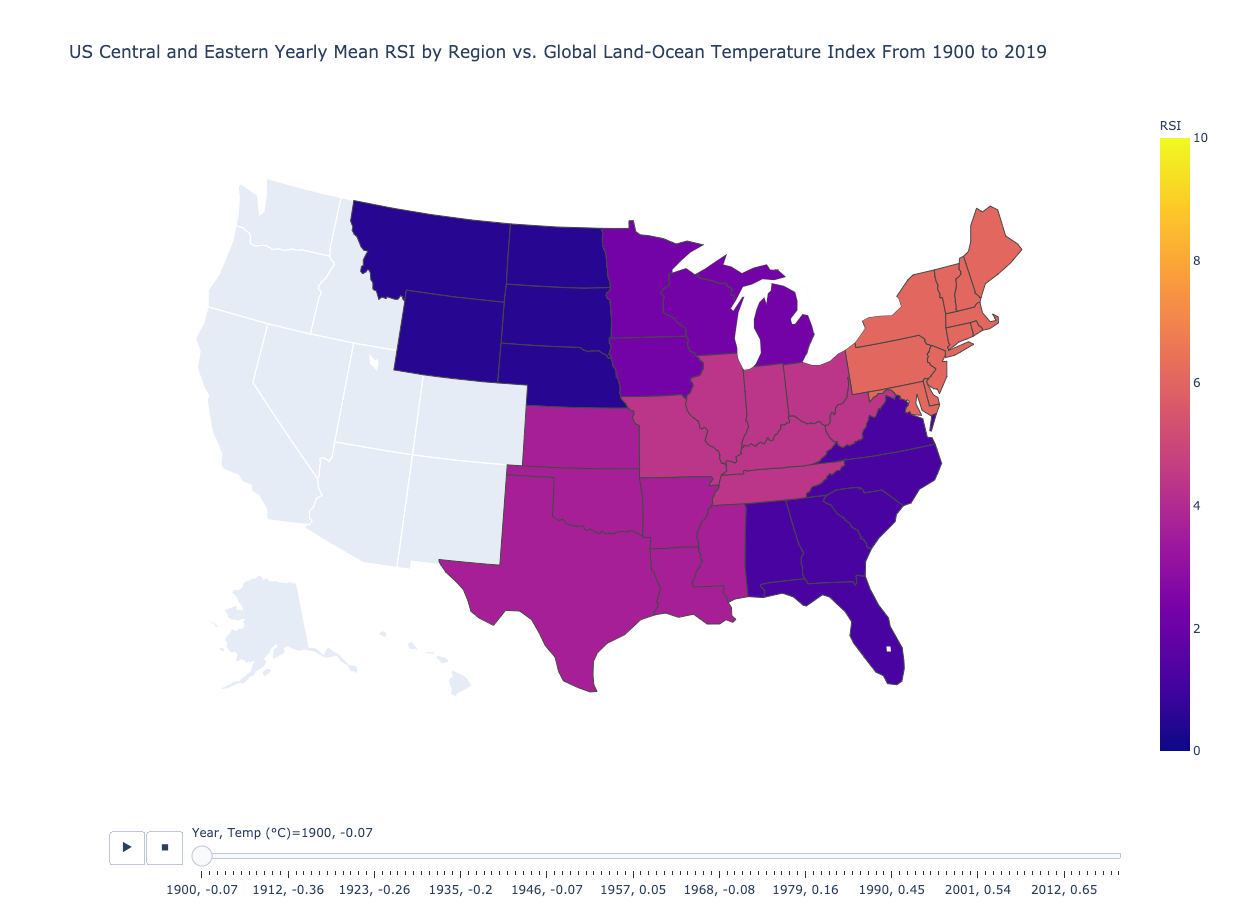
\includegraphics[scale=.35]{choropleth.png}
    \caption{A choropleth map showing the US central and eastern regions RSI with global temperatures over the years 1900-2019.}
    \label{fig:my_label}
\end{figure}

\newpage

\begin{figure}[h]
    \centering 
    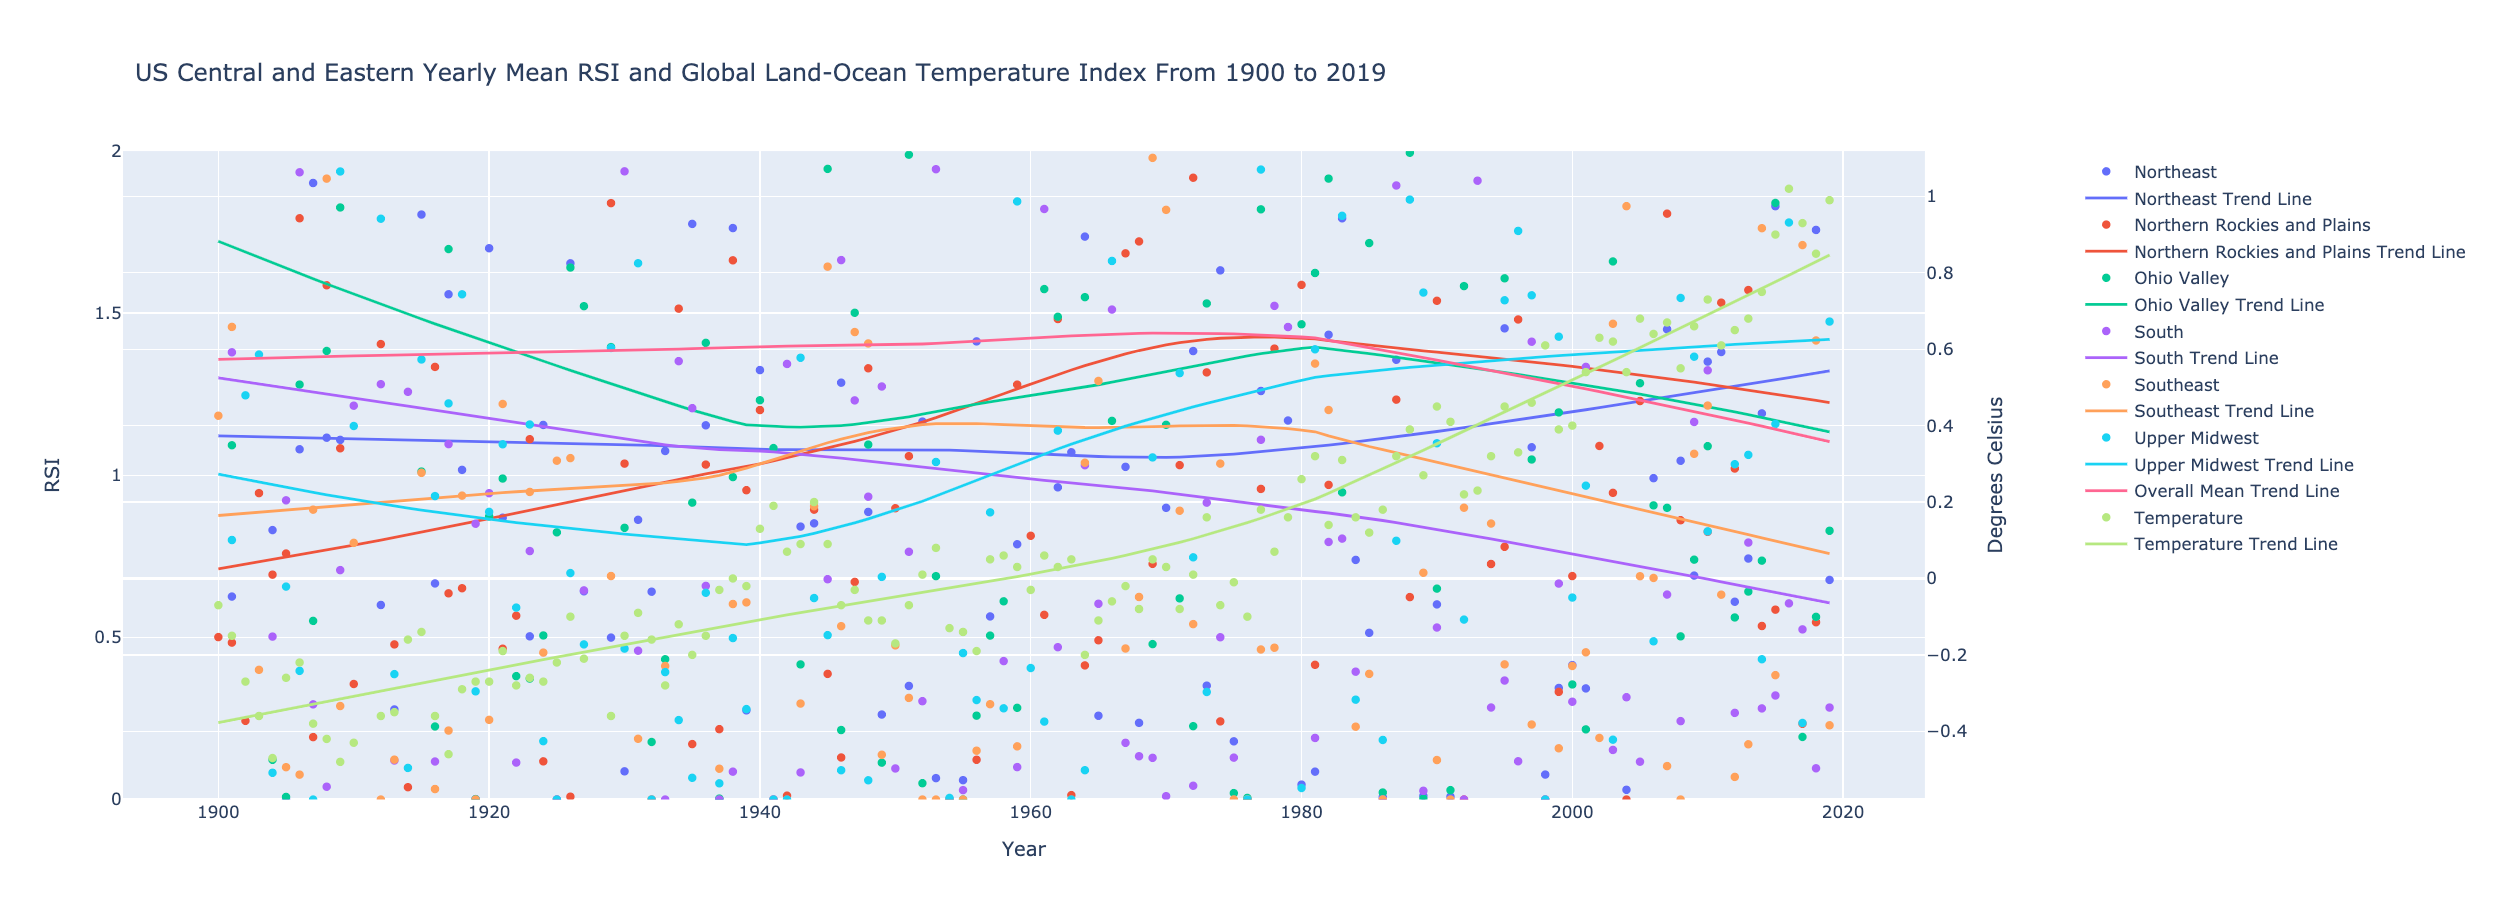
\includegraphics[scale=.2]{year_comparison_scatter_plot_wide.png}
    \caption{A scatter plot mapping the RSI of US central and eastern regions with global temperatures over the years 1900-2019.}
    \label{fig:my_label}
    \end{figure}
\begin{figure}[h]
    \centering
    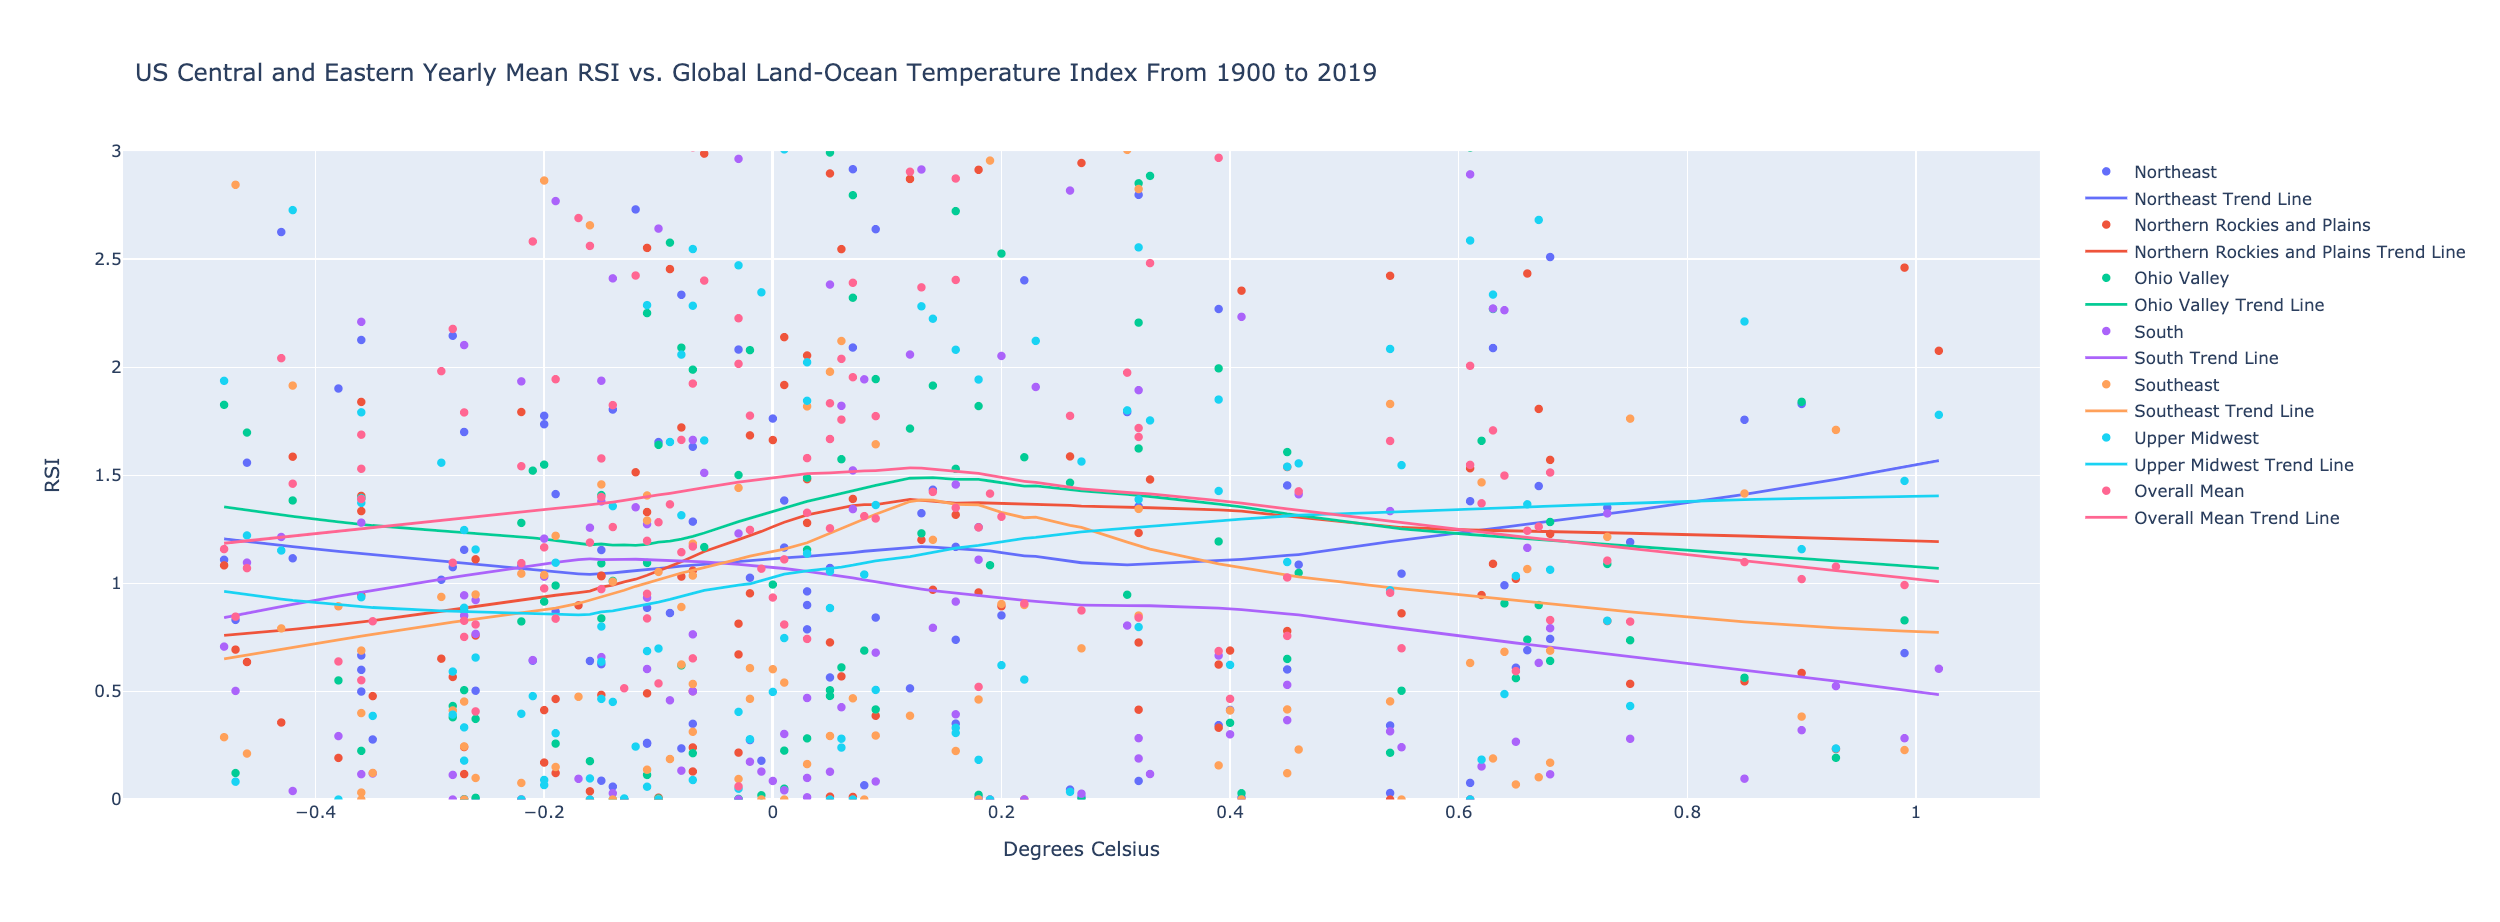
\includegraphics[scale=.2]{correlation_scatter_plot_wide.png}
    \caption{A scatter plot showing the correlation between the RSI of US central and eastern regions and increasing global temperatures.}
    \label{fig:my_label}
\end{figure}



\section*{Changes from Project Proposal}
For the most part, our goal with this project has remained unchanged from the project proposal. That being said, there are several notable changes to our research question and computational plan. We changed our research question to be more specific to the data-sets that we have, noting that our snowfall data is categorized by regional impact in the United States and being more specific in saying ``increasing global temperatures" rather than just ``climate change". Also, at the time of submitting our proposal, we hadn't fully decided how we wanted to visualize our data. Since then, we decided to do so in three ways: first, with our choropleth created in \texttt{plotly} which shows snowfall impacts on a yearly basis; second, with our scatter plot which shows the individual RSI data points for each region as well as trend lines for each region and for temperature over time; third, with another scatter plot which plots our calculated regression lines between each region's snowfall, mean snowfall, and temperature.

\section*{Discussion}
Our program generates three diagrams to find a correlation between the impact of snowfall and global temperature change within the following regions of the US provided in the NOAA dataset: Northeast, Northern Rockies and Plains, Ohio Valley, South, Southeast, and Upper Midwest.

Our Choropleth shows the RSI (Regional Snowfall Index) of these regions throughout the years 1900 to 2019. High RSI values (6-10) are regions that were affected by major snowfall, illustrated by hot colours like magenta, orange, and yellow. Conversely, low RSI values (1-6) indicate notable or significant snowfall displayed by cool colours like purple and dark blue. Here, it is evident that the years 1900 to 2000 have a consistent pattern of low RSI along with many years impacted by a high RSI. However, around the 2000’s and later there are consecutive years where the RSI is low and rarely impacted with major snowfall with two exceptions in the early 2000’s and somewhere around 2015. As the years pass, the average global temperature continuously becomes warmer (except between 1957-1968 where the global temperature became colder with essentially the same RSI values) and with the 2000’s being the warmest, we can conclude that there possible is a correlation between increasing temperature levels and snowfall impact at least in recent years. 

Our Year Comparison Scatterplot maps the same information as our Choropleth and are using trend lines to allow us to better see patterns and come to conclusions. Each line in the graph represents a region as well as the temperature and an overall mean for the RSI. Throughout the years, the average temperature anomaly continuously increases. The South, Southeast, Northeast Rockies, and Ohio Valley all have a decreasing RSI during the 1980’s to 2019, where the temperature started to dramatically become warmer. However, the Northeast and Upper Midwest regions both increase in RSI. Moreover, some regions have an RSI that grows between the 1940’s and mid 1970’s like the Upper Midwest and the Ohio Valley after having a dramatic decrease in the early 1900’s. There are also regions that stayed seemingly constant like the Northeast and Northern Rockies and Plain from the 1900’s up to the 1980’s. In fact, the only region to consistently decrease in RSI throughout the years as the global temperature increases is the South. There seemingly is no consistent trend. Only after the 1980’s, when the global temperature starts to significantly increase, does most of the regions snowfall impact decrease. The following graph was made based on this scatterplot, showing only the trend lines of the temperature anomaly and average RSI from 1900-2019:

\begin{figure}[h]
    \centering 
    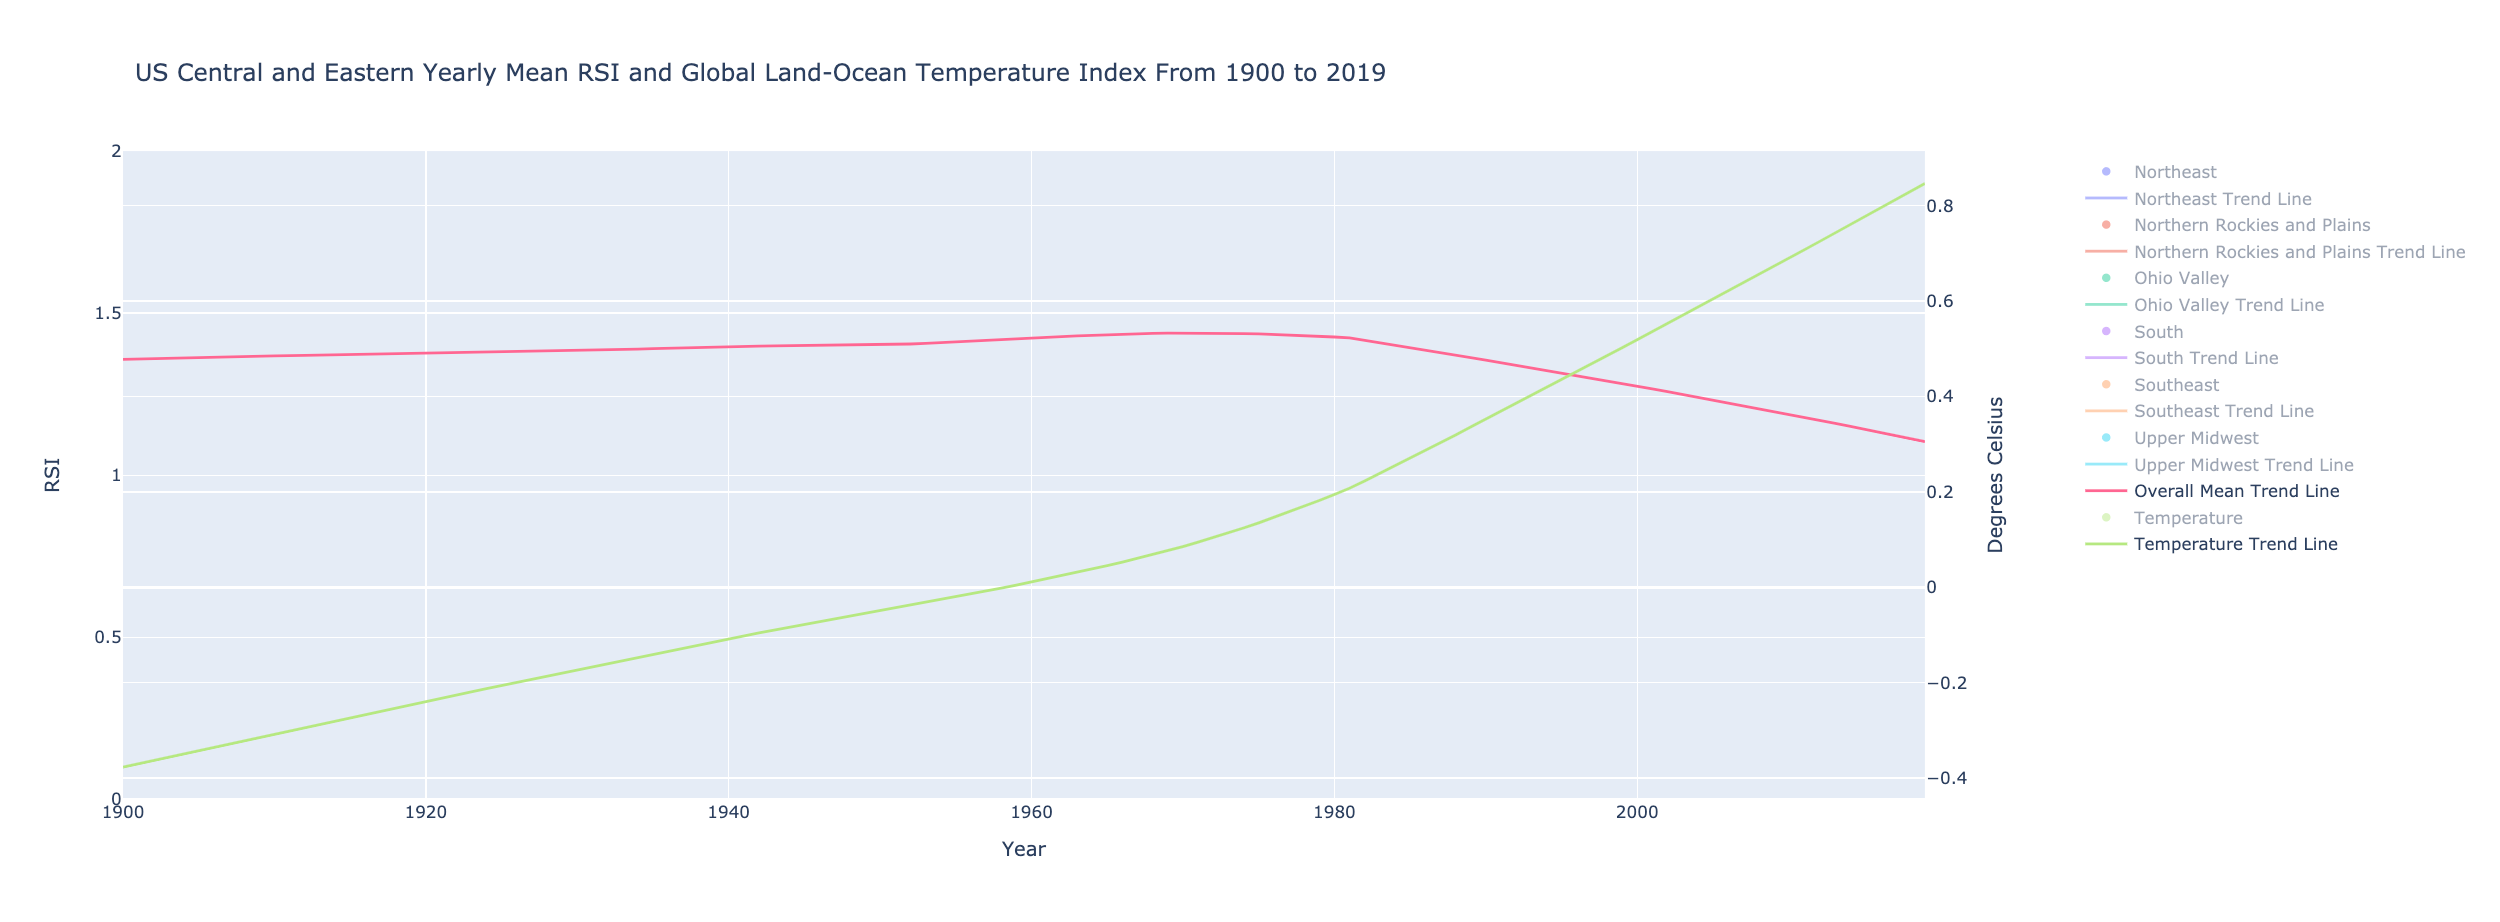
\includegraphics[scale=.2]{year_comparison_scatter_plot_summary_wide.png}
    \caption{A graph showing the trend lines of the RSI of US central and eastern regions with global temperatures over the years 1900-2019.}
    \label{fig:my_label}
\end{figure}

Although there is no continuous pattern, we can conclude that there may be a correlation with warmer temperatures and snowfall impact due to the graphs after 1980.

Our final diagram is a Correlation Scatterplot mapping only the RSI of the climate regions and the global temperature. Like the previous scatterplot, each line represents a region along with an overall RSI mean. As expected, most regions have an RSI that decreases at a certain point, that point being 0.2 degrees. This matches the year we established beforehand, 1980, which had a 0.26 temperature increase and where the RSI began to trend downwards in our other two diagrams. Before this, the regions were split in half with one half having an RSI decrease and another having an increase between temperatures -0.4 and 0.2. These trends can also be shown on a graph we created that compares the average RSI values with the temperature anomaly using LOWESS smoothing:

\begin{figure}[h]
    \centering 
    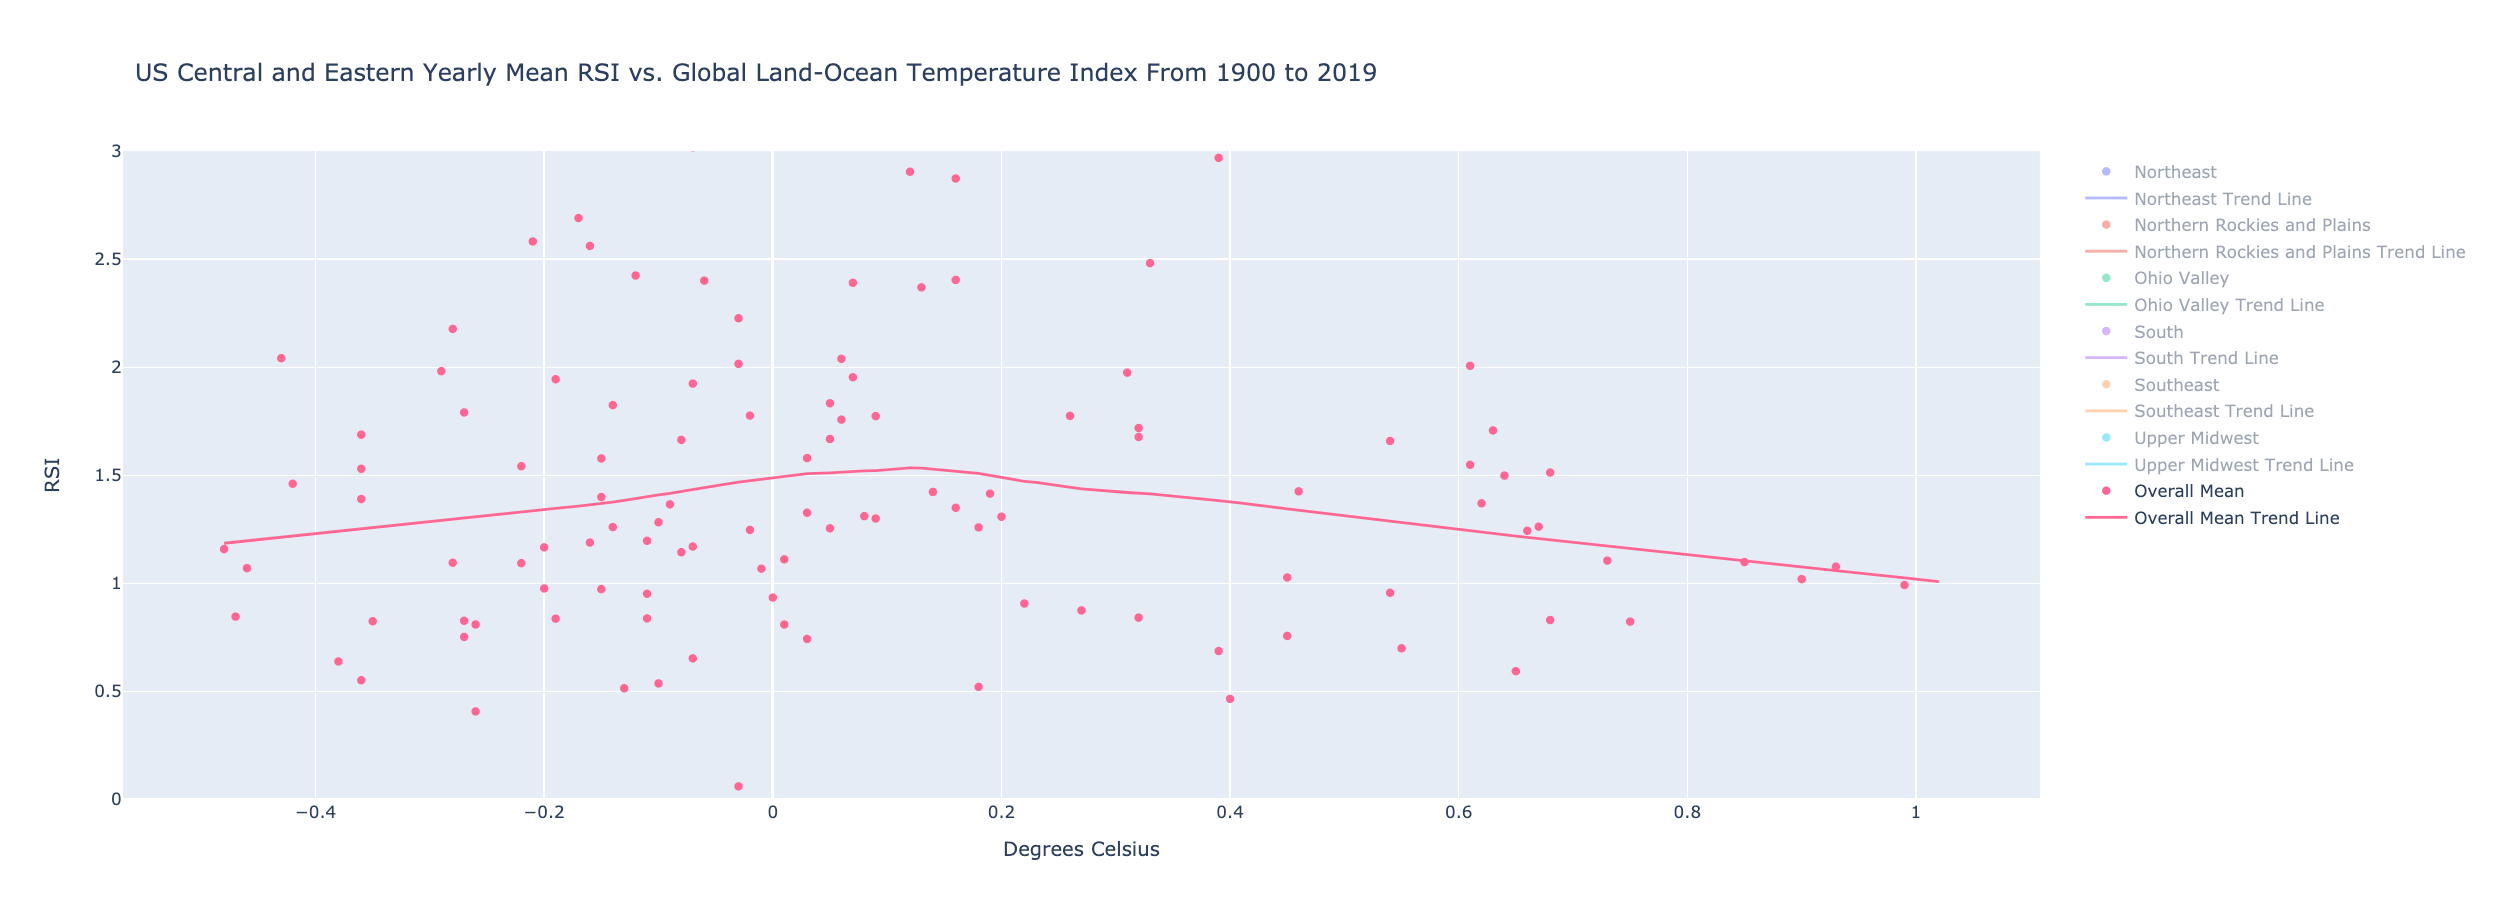
\includegraphics[scale=.2]{correlation_scatter_plot_summary_wide.png}
    \caption{A graph comparing the average RSI of US central and eastern regions with increasing global temperatures.}
    \label{fig:my_label}
\end{figure}


This graph shows the RSI does decrease around a 0.2 temperature increase. Prior to this, there is a slight increase in RSI due to the halved regions, as seen in the Correlation Scatterplot. We can again conclude there is possibly a correlation between increasing global temperatures and snowfall impact due to the graphs after a temperature increase of 0.2.


To conclude, our research has shown that there is a possible correlation between rising global temperatures and the RSI data from these US climate regions. One of the major constraints we faced was the scope of the data-sets we were working with, which did not contain any information about western US regions. In terms of obstacles with libraries used, \texttt{pandas} was initially a bit of a challenge to adapt to. However, after some research, DataFrame manipulations that were expected to take multiple for loops were reduced to a single line. As well, deciding between \texttt{plotly express} and \texttt{plotly graphing objects} was initially difficult, but as we familiarized ourselves with the capabilities of each, we determined that we could use both to suit our graphing needs. In terms of next steps, we think that our visualizations could be applied to future weather data to further clarify whether there is correlation between rising global temperatures and RSI values.

\section*{References}

Getting Started with Plotly. (n.d.). Plotly.com. \url{https://plotly.com/python/getting-started/}

Mote, P. W., Li, S., Lettenmaier, D. P., Xiao, M., \& Engel, R. (2018). Dramatic declines in snowpack in the western US. Npj Climate and Atmospheric Science, 1(1). doi:10.1038/s41612-018-0012-1
% https://www.nature.com/articles/s41612-018-0012-1

NASA/GISS (2019). Global Land-Ocean Temperature Index [Data set]. NASA. \url{https://data.giss.nasa.gov/gistemp/graphs/graph\_data/Global\_Mean\_Estimates\_based\_on\_Land\_and\_Ocean\_Data/graph.txt}

NASA (2020). Global Surface Temperature. Retrieved December 13, 2020, from \url{https://climate.nasa.gov/vital-signs/global-temperature/}

NOAA (2019). Regional Snowfall Index [Data set]. NOAA. \url{https://www.ncei.noaa.gov/metadata/geoportal/rest/metadata/item/gov.noaa.ncdc:C00465/html}
% https://www.ncei.noaa.gov/metadata/geoportal/rest/metadata/item/gov.noaa.ncdc:C00465/html

Schmunk, R. B. (2020, January 14). Data.GISS: GISTEMP -- Frequently Asked Questions. Data.Giss.Nasa.Gov. \url{https://data.giss.nasa.gov/gistemp/faq/#q103}
% https://data.giss.nasa.gov/gistemp/faq/#q103

User Guide — pandas 1.0.1 documentation. (2014). Pydata.Org. \url{https://pandas.pydata.org/docs/user_guide/index.html}

% NOTE: LaTeX does have a built-in way of generating references automatically,
% but it's a bit tricky to use so we STRONGLY recommend writing your references
% manually, using a standard academic format like APA or MLA.
% (E.g., https://owl.purdue.edu/owl/research_and_citation/apa_style/apa_formatting_and_style_guide/general_format.html)

\end{document}

